{
\usebackgroundtemplate{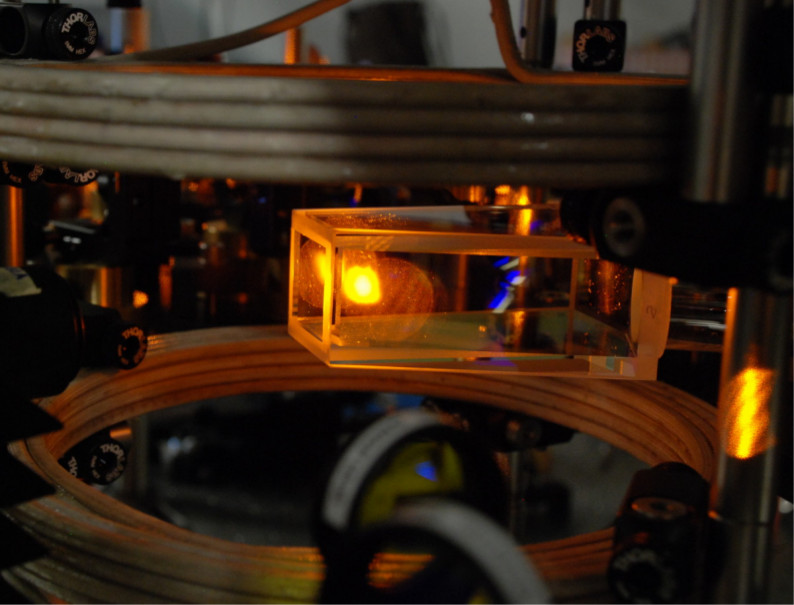
\includegraphics[width=\paperwidth]{Figures/MOT-picture.jpg}}
\begin{frame}<1-4>[t,plain,label=Outline]


\begin{minipage}[c][0.5\textheight][c]{\linewidth}
	\setbeamercolor{title}{fg=white,bg=bellblue}
	\only<1-3>{\pgfsetfillopacity{0.75}}
	\only<4->{\pgfsetfillopacity{0.35}}
	\hfill
	\begin{beamercolorbox}[wd=0.75\linewidth,center,colsep=0.5em,rounded=false]{title}
		\begin{center}
		\only<1-4>{\circled{white}{0.75}{1}\\}
		\only<5->{\circled{white}{0.35}{1}\\} 
		\vspace{1.5em}
		\textbf{Introduction} \\
		\vspace{1.5em}
		\end{center}
	\end{beamercolorbox}
	\hfill\hfill
\end{minipage}

\only<2->{
\begin{minipage}[c][0.5\textheight][c]{\linewidth}
	\setbeamercolor{title}{fg=white,bg=bellblue}
	\only<2,3>{\pgfsetfillopacity{0.75}}
	\only<5->{\pgfsetfillopacity{0.35}}
	\hfill
	\begin{beamercolorbox}[wd=0.75\linewidth,center,colsep=1em,rounded=false]{title}
		\begin{center}
		\only<2,3,5>{\circled{white}{0.75}{2}\\}
		\only<4,6->{\circled{white}{0.35}{2}\\}
		\vspace{1.5em}
		\textbf{Spin-Dipole polarizability} \\
		\vspace{1em}
		\end{center}
	\end{beamercolorbox}
	\hfill\hfill
\end{minipage}
}


\end{frame}
}
